\section{Experiments}
\label{sec:experiments}

We organize our experiments into four progressive approaches. The Baseline establishes reference points for both the healthy-versus-depressed task and the core bipolar-versus-unipolar task using the CNN-LSTM described in Section~\ref{sec:methods}. Approach~1 investigates class imbalance as the primary obstacle by replacing synthetic oversampling with downsampling. Approach~2 tests four alternative neural architectures to determine whether model design is the limiting factor. Approach~3 conducts a comprehensive diagnostic analysis using classical machine learning \cite{pedregosa2011sklearn}, direct statistical testing, and visualization to probe the fundamental signal structure of the data. All hyperparameter configurations are evaluated using grid search \cite{bergstra2012random}.

% ============================================================
\subsection{Baseline}
% ============================================================

We begin with two foundational experiments using the 1D-CNN-LSTM architecture. The first validates the full pipeline on a simpler binary classification task before tackling the core challenge. The second directly addresses the primary research question of separating bipolar from unipolar depression. These two experiments together serve as reference points against which all subsequent approaches are compared.

\subsubsection{Experiment 1: Healthy versus Depressed.}

\paragraph{Approach.}
Before confronting the harder differential diagnosis task, we validate whether the 1D-CNN-LSTM pipeline can extract meaningful features from raw actigraphy to separate mood-disorder patients from healthy controls. This binary classification problem is well studied in the literature \cite{garcia2018depresjon,jakobsen2020applying}, allowing us to benchmark our approach against established results. We hypothesize that depressed individuals will exhibit measurably reduced and fragmented motor activity patterns that the CNN-LSTM can learn to distinguish from healthy movement profiles, and that the end-to-end approach on raw sequences will be competitive with prior work using hand-crafted features.

\paragraph{Methodology.}
All 55 participants are included: 32 healthy controls and 23 mood-disorder patients. The 80/10/10 participant-level stratified split yields a training set of 44 participants and 20,385 windows, a validation set of 5 participants and 2,326 windows, and a test set of 6 participants and 2,190 windows. The standard CNN-LSTM architecture is trained with class-weighted cross-entropy loss. The following hyperparameters are explored:
\begin{itemize}[nosep]
  \item Learning rate: $\{10^{-3}, 5 \times 10^{-4}, 10^{-4}\}$
  \item Weight decay: $\{10^{-4}, 10^{-3}\}$
  \item Dropout probability: $\{0.3, 0.4, 0.5\}$
  \item Class weight: inverse frequency vs.\ equal weights
\end{itemize}
Best configuration: lr $= 10^{-3}$, wd $= 10^{-4}$, dropout $= 0.4$, inverse frequency weighting. Evaluation metric: macro-averaged F1-Score.

\paragraph{Results.}
Table~\ref{tab:exp1_results} reports the performance of our CNN-LSTM against prior work on the same dataset.

\begin{table}[H]
\centering
\caption{Experiment 1: Healthy vs.\ Depressed, compared with prior work.}
\label{tab:exp1_results}
\begin{tabular}{lcccc}
\toprule
\textbf{Method} & \textbf{Acc.} & \textbf{Sensitivity} & \textbf{Specificity} & \textbf{F1} \\
\midrule
Random Forest \cite{garcia2018depresjon} & 0.71 & 0.57 & 0.81 & 0.61 \\
Weighted CNN \cite{jakobsen2020applying} & 0.73 & 0.65 & 0.78 & 0.66 \\
DNN + SMOTE \cite{jakobsen2020applying} & 0.83 & 0.82 & 0.84 & 0.82 \\
\textbf{CNN-LSTM (Ours)} & \textbf{0.534} & \textbf{0.458} & \textbf{0.590} & \textbf{0.516} \\
\bottomrule
\end{tabular}
\end{table}

\begin{figure}[H]
\centering
\begin{minipage}{0.48\linewidth}
  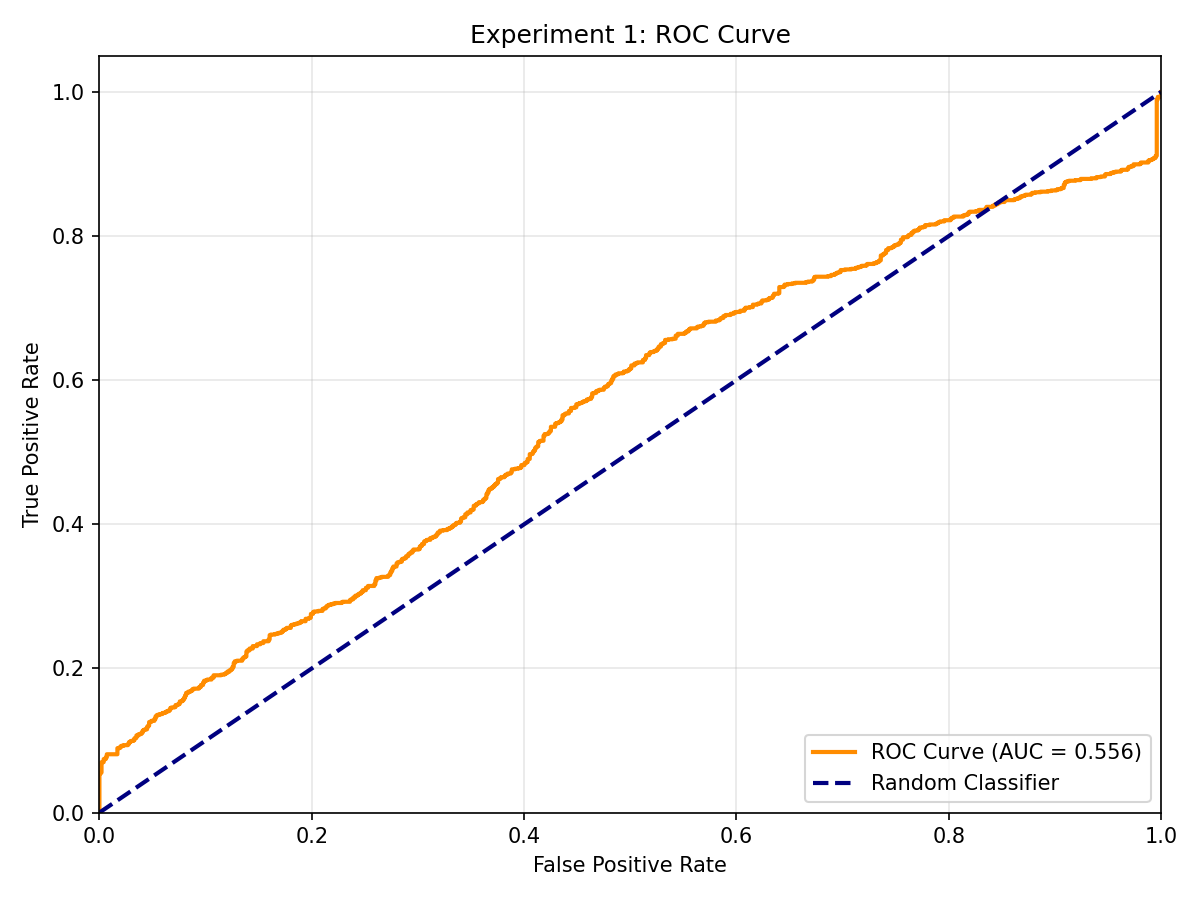
\includegraphics[width=\linewidth]{images/exp1_roc_curve.png}
\end{minipage}
\hfill
\begin{minipage}{0.48\linewidth}
  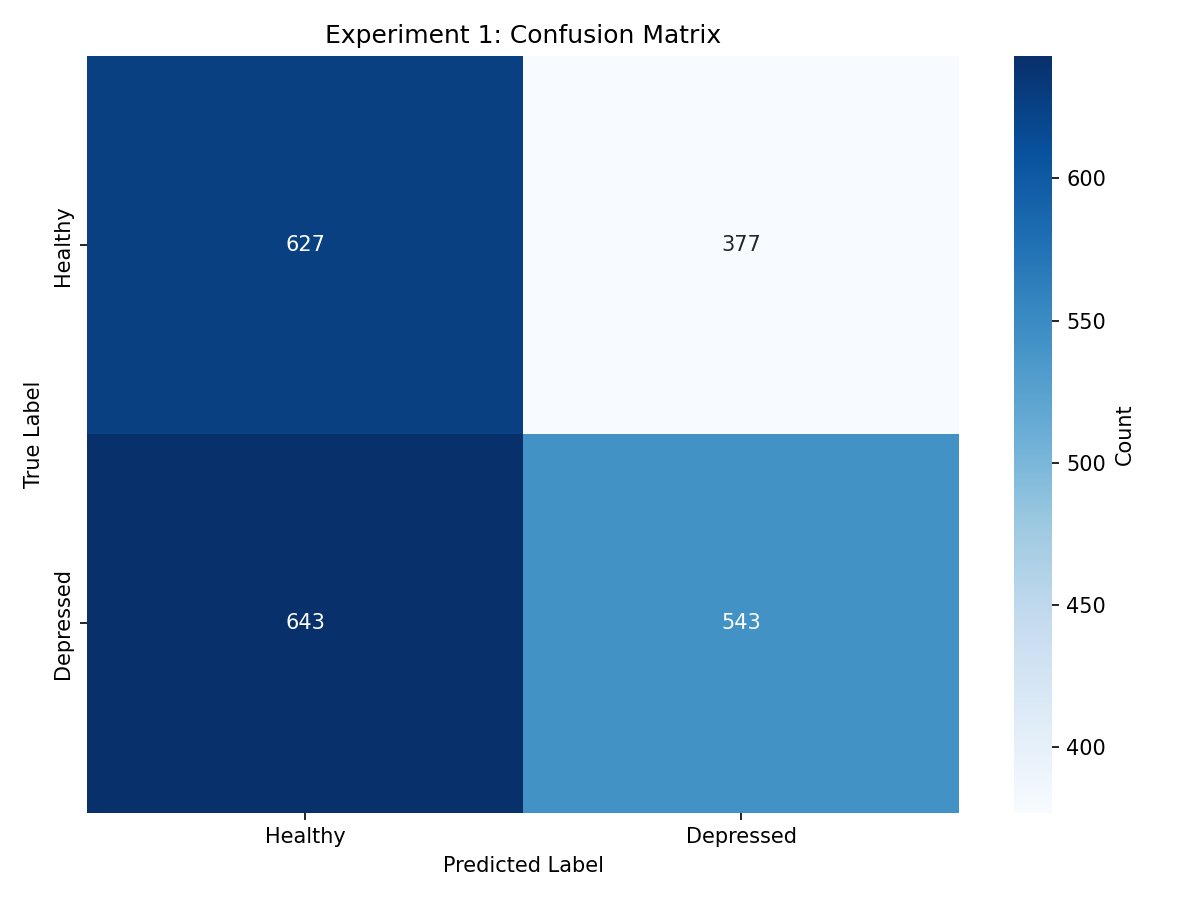
\includegraphics[width=\linewidth]{images/exp1_confusion_matrix.png}
\end{minipage}
\caption{Experiment 1 results. \textit{Left:} ROC curve (AUC = 0.556), marginally above the random classifier diagonal. \textit{Right:} Confusion matrix showing near-balanced misclassification between healthy and depressed classes.}
\label{fig:exp1}
\end{figure}

\paragraph{Conclusion.}
The hypothesis that end-to-end CNN-LSTM would be competitive with prior hand-crafted-feature approaches is not supported. The model achieves F1 = 0.516, well below the DNN+SMOTE baseline of 0.82. This suggests that raw 1,440-minute sequences are difficult to learn from at this dataset scale: the model learns some signal (AUC = 0.556) but cannot generalize reliably, likely because the 223K-parameter architecture is severely over-parameterized relative to the 44 available training participants.

\subsubsection{Experiment 2: Bipolar versus Unipolar Depression with SMOTE.}

\paragraph{Approach.}
We now turn to the core clinical challenge: distinguishing bipolar disorder from unipolar depression using only motor activity. This experiment isolates the 23 condition participants (8 bipolar, 15 unipolar) and trains the CNN-LSTM to make the differential diagnosis. The 8:15 class imbalance poses a substantial challenge, addressed here using SMOTE \cite{chawla2002smote} applied at the window level alongside class-weighted loss. We hypothesize that the LSTM's ability to integrate multi-day circadian rhythm patterns will provide sufficient signal to make this distinction, and that SMOTE will generate sufficiently realistic synthetic minority-class examples to prevent majority-class collapse.

\paragraph{Methodology.}
The 23 condition participants are split at the participant level (80/10/10). SMOTE is applied to the training windows only to avoid leakage into validation or test sets. Hyperparameters explored:
\begin{itemize}[nosep]
  \item SMOTE nearest neighbors $k$: $\{3, 5, 7\}$
  \item Minority class loss weight $\alpha$: $\{0.65, 0.70, 0.75\}$
  \item Learning rate: $\{10^{-3}, 5 \times 10^{-4}\}$
  \item Dropout probability: $\{0.3, 0.4\}$
\end{itemize}
Best configuration: $k = 5$, $\alpha = 0.70$, lr $= 10^{-3}$, dropout $= 0.4$. Primary evaluation metric: ROC-AUC \cite{fawcett2006roc}.

\paragraph{Results.}
Table~\ref{tab:exp2_results} reports the test-set performance metrics and confusion matrix breakdown.

\begin{table}[H]
\centering
\caption{Experiment 2 results and confusion matrix (rows: actual, columns: predicted).}
\label{tab:exp2_results}
\begin{tabular}{lc}
\toprule
\textbf{Metric} & \textbf{Value} \\
\midrule
Accuracy & 88.01\% \\
Precision & 100.00\% \\
F1-Score & 0.936 \\
Bipolar cases detected & 0 / 121 \\
\midrule
Pred.\ Unipolar / Pred.\ Bipolar (Actual Unipolar) & 888 / 0 \\
Pred.\ Unipolar / Pred.\ Bipolar (Actual Bipolar) & 121 / 0 \\
\bottomrule
\end{tabular}
\end{table}

\begin{figure}[H]
\centering
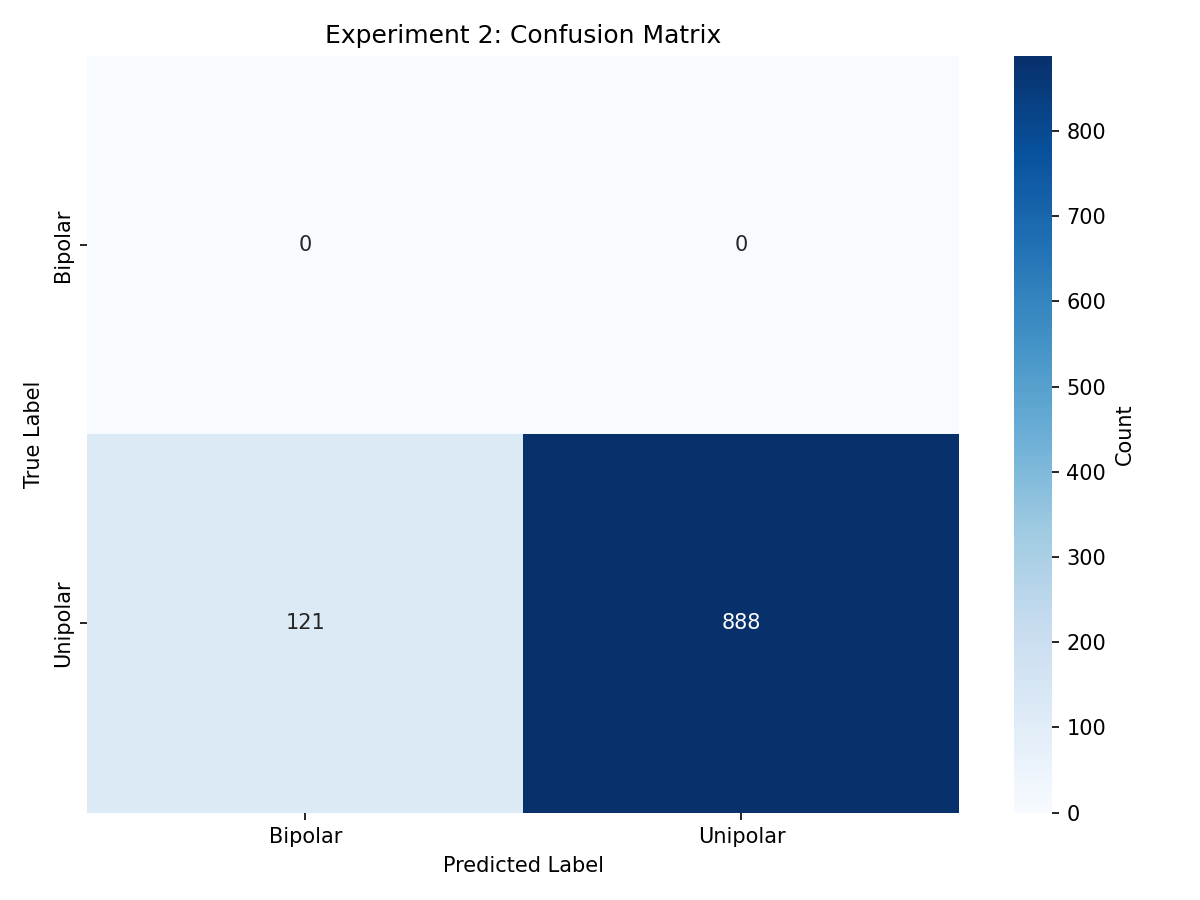
\includegraphics[width=0.7\linewidth]{images/exp2_confusion_matrix.png}
\caption{Experiment 2 confusion matrix. The model predicts every window as unipolar (0 bipolar cases detected), achieving 88\% accuracy purely through majority-class collapse.}
\label{fig:exp2_cm}
\end{figure}

\paragraph{Conclusion.}
Despite reporting 88\% accuracy, the model predicts every test window as unipolar, detecting zero bipolar cases. The high accuracy figure is entirely explained by the 888:121 class distribution in the test set. SMOTE did not prevent majority-class collapse; the synthetic windows appear not to have provided the model with sufficient discriminative signal. The hypothesis is not supported. The failure of SMOTE motivates Approach~1.

% ============================================================
\subsection{Approach 1: Balanced Dataset via Downsampling}
% ============================================================

Having observed that SMOTE does not prevent majority-class collapse, we investigate whether class imbalance itself is the fundamental obstacle. Rather than artificially inflating the minority class, we reduce the majority class through random downsampling to create a natural 1:1 training balance. We hypothesize that class imbalance, rather than signal weakness, is the primary obstacle to bipolar-unipolar differentiation, and that training on a balanced dataset will allow the model to learn genuine discriminative features for both classes.

\subsubsection{Experiment: CNN-LSTM with Balanced Downsampling.}

\paragraph{Approach.}
We apply the same 1D-CNN-LSTM architecture to a training set in which unipolar windows are randomly downsampled to match the count of bipolar windows, creating a 1:1 class ratio. If balancing is the key missing ingredient, we should observe meaningful improvement in bipolar case detection.

\paragraph{Methodology.}
Downsampling is applied only to the training set after the participant-level split. Hyperparameters explored:
\begin{itemize}[nosep]
  \item Learning rate: $\{10^{-3}, 5 \times 10^{-4}\}$
  \item Weight decay: $\{10^{-4}, 10^{-3}\}$
  \item Dropout probability: $\{0.3, 0.4, 0.5\}$
  \item Batch size: $\{32, 64\}$
\end{itemize}
Best configuration: lr $= 10^{-3}$, wd $= 10^{-4}$, dropout $= 0.4$, batch size $= 32$.

\paragraph{Results.}
Table~\ref{tab:approach1_results} compares Approach~1 against the Baseline Experiment~2.

\begin{table}[H]
\centering
\caption{Approach 1 results: CNN-LSTM with balanced downsampling vs.\ Baseline Exp~2.}
\label{tab:approach1_results}
\begin{tabular}{lcc}
\toprule
\textbf{Metric} & \textbf{Approach 1} & \textbf{Baseline Exp 2} \\
\midrule
Accuracy & 65.41\% & 88.01\%$\dagger$ \\
F1-Score & 0.791 & 0.936$\dagger$ \\
Bipolar Detected & 0 / 349 & 0 / 121 \\
\bottomrule
\multicolumn{3}{l}{\footnotesize $\dagger$ Illusory; majority-class collapse.}
\end{tabular}
\end{table}

% Figure dropped: covered comprehensively by the cross-approach comparison (Fig.~\ref{fig:all_approaches}).

\paragraph{Conclusion.}
Despite perfect 1:1 class balance during training, the model still collapses to predicting all test windows as unipolar, with zero bipolar cases detected across 349 bipolar test windows. The hypothesis that class imbalance is the root cause is definitively not supported. This result shifts our working hypothesis to a fundamental signal-weakness problem: the motor activity patterns of bipolar and unipolar patients during depressive episodes may not be meaningfully different, regardless of how the training set is composed.

% ============================================================
\subsection{Approach 2: Alternative Neural Architectures}
% ============================================================

With class imbalance ruled out as the primary obstacle, we investigate whether the architectural design of our CNN-LSTM is the limiting factor. We train four alternative neural architectures on the balanced dataset from Approach~1: Bidirectional LSTM, Attention-enhanced LSTM, RNN-LSTM hybrid, and an Ensemble of three CNN-LSTM models. We hypothesize that one or more of these architectural extensions will capture diagnostic signal that the standard unidirectional CNN-LSTM misses, through broader temporal context (BiLSTM), selective focus on relevant time segments (Attention), faster local pattern capture (RNN-LSTM), or variance reduction through model averaging (Ensemble).

\subsubsection{Bidirectional LSTM.}

\paragraph{Approach.}
A standard LSTM processes sequences from left to right, potentially missing diagnostic context from future time steps. We extend the architecture with bidirectional LSTM layers \cite{graves2005bilstm}, processing each sequence in both temporal directions simultaneously. We hypothesize that patterns in activity immediately following a sleep period carry diagnostic information only accessible when sequences are processed in both directions.

\paragraph{Methodology.}
The standard LSTM is replaced with a bidirectional LSTM of 128 hidden units per direction. Hyperparameters explored:
\begin{itemize}[nosep]
  \item Learning rate: $\{10^{-3}, 5 \times 10^{-4}, 10^{-4}\}$
  \item Dropout probability: $\{0.3, 0.4, 0.5\}$
  \item Hidden units per direction: $\{64, 128\}$
\end{itemize}
Best configuration: lr $= 10^{-3}$, dropout $= 0.4$, 128 hidden units per direction.

\paragraph{Results.}
Table~\ref{tab:approach2a_results} compares the BiLSTM against Approach~1.

\begin{table}[H]
\centering
\caption{Approach 2a: BiLSTM vs.\ Approach~1 baseline.}
\label{tab:approach2a_results}
\begin{tabular}{lcc}
\toprule
\textbf{Metric} & \textbf{BiLSTM} & \textbf{Approach 1} \\
\midrule
Accuracy & 55.40\% & 65.41\% \\
F1-Score & 0.713 & 0.791 \\
Bipolar Detected & 0 / 349 & 0 / 349 \\
\bottomrule
\end{tabular}
\end{table}

\paragraph{Conclusion.}
The bidirectional architecture performs worse than the standard CNN-LSTM (55.4\% vs 65.4\%) and again detects zero bipolar cases. Additional parameters from the second LSTM direction appear to increase overfitting without providing corresponding discriminative signal. The hypothesis is not supported.

\subsubsection{Attention-Enhanced LSTM.}

\paragraph{Approach.}
An attention mechanism \cite{bahdanau2015attention} allows the model to assign a learned weight to each time step, enabling concentration on diagnostically relevant moments within a 24-hour window, such as sleep-onset timing. We hypothesize that certain time-of-day periods carry disproportionate diagnostic weight that an attention mechanism will learn to identify.

\paragraph{Methodology.}
A self-attention layer is inserted between the LSTM output and the classification head, with the CNN blocks and FC head unchanged. Hyperparameters explored:
\begin{itemize}[nosep]
  \item Attention dimension: $\{32, 64, 128\}$
  \item Learning rate: $\{10^{-3}, 5 \times 10^{-4}\}$
  \item Dropout probability: $\{0.3, 0.4, 0.5\}$
\end{itemize}
Best configuration: attention dim $= 64$, lr $= 5 \times 10^{-4}$, dropout $= 0.4$.

\paragraph{Results.}
Table~\ref{tab:approach2b_results} compares the Attention LSTM against Approach~1.

\begin{table}[H]
\centering
\caption{Approach 2b: Attention LSTM vs.\ Approach~1 baseline.}
\label{tab:approach2b_results}
\begin{tabular}{lcc}
\toprule
\textbf{Metric} & \textbf{Attention LSTM} & \textbf{Approach 1} \\
\midrule
Accuracy & 48.17\% & 65.41\% \\
F1-Score & 0.650 & 0.791 \\
Bipolar Detected & 0 / 523 & 0 / 349 \\
\bottomrule
\end{tabular}
\end{table}

\paragraph{Conclusion.}
The Attention LSTM is the worst-performing architecture in the project (48.17\%). With only 8 bipolar participants, the attention mechanism does not receive sufficient signal to learn meaningful diagnostic weights. The hypothesis is not supported.

\subsubsection{RNN-LSTM Hybrid.}

\paragraph{Approach.}
A hybrid architecture combining vanilla RNN cells with an LSTM layer offers a distinct inductive bias: RNN cells capture rapid local state transitions while the downstream LSTM integrates this information over longer time horizons. We hypothesize that the fast transition detection of the RNN layer might surface short-duration activity events that carry diagnostic signal.

\paragraph{Methodology.}
A stacked RNN layer is added before the LSTM, with convolutional blocks removed. Hyperparameters explored:
\begin{itemize}[nosep]
  \item RNN hidden size: $\{64, 128\}$; LSTM hidden size: $\{64, 128\}$
  \item Learning rate: $\{10^{-3}, 10^{-4}\}$; Dropout: $\{0.3, 0.4\}$
\end{itemize}
Training was terminated early due to sustained validation loss oscillation consistent with gradient instability.

\paragraph{Results.}
Table~\ref{tab:approach2c_results} summarizes the training behavior that led to early termination.

\begin{table}[H]
\centering
\caption{Approach 2c: RNN-LSTM Hybrid. Training accuracy reflects overfitting; results discarded.}
\label{tab:approach2c_results}
\begin{tabular}{lcc}
\toprule
\textbf{Metric} & \textbf{RNN-LSTM} & \textbf{Approach 1} \\
\midrule
Training Accuracy & 100.0\%$\ddagger$ & 65.41\% \\
Validation Behavior & Oscillating & Stable \\
Status & Discarded & Valid \\
\bottomrule
\multicolumn{3}{l}{\footnotesize $\ddagger$ Overfitting; validation loss did not converge.}
\end{tabular}
\end{table}

\paragraph{Conclusion.}
The RNN-LSTM exhibits catastrophic overfitting and is discarded as unreliable. The failure further underscores that model capacity is a constraint at this dataset size.

\subsubsection{Ensemble Model.}

\paragraph{Approach.}
Ensemble methods aggregate predictions from multiple independently trained models, reducing variance and potentially surfacing weak signals that individual models miss. We train three CNN-LSTM models with different random seeds and combine their output probabilities via soft voting. We hypothesize that variance reduction through ensembling might expose the weak bipolar signal that individual models independently fail to detect.

\paragraph{Methodology.}
Three CNN-LSTM models are trained with seeds $\{42, 123, 456\}$ on the balanced dataset from Approach~1, using the same best configuration. Soft voting on class probabilities is the primary aggregation strategy; hard voting is also evaluated for comparison.

\paragraph{Results.}
Table~\ref{tab:approach2d_results} compares the Ensemble against the best individual CNN-LSTM.

\begin{table}[H]
\centering
\caption{Approach 2d: Ensemble Model vs.\ best individual CNN-LSTM.}
\label{tab:approach2d_results}
\begin{tabular}{lcc}
\toprule
\textbf{Metric} & \textbf{Ensemble} & \textbf{Approach 1} \\
\midrule
Accuracy & 59.66\% & 65.41\% \\
F1-Score & 0.747 & 0.791 \\
Bipolar Detected & 0 / 407 & 0 / 349 \\
\bottomrule
\end{tabular}
\end{table}

\begin{figure}[H]
\centering
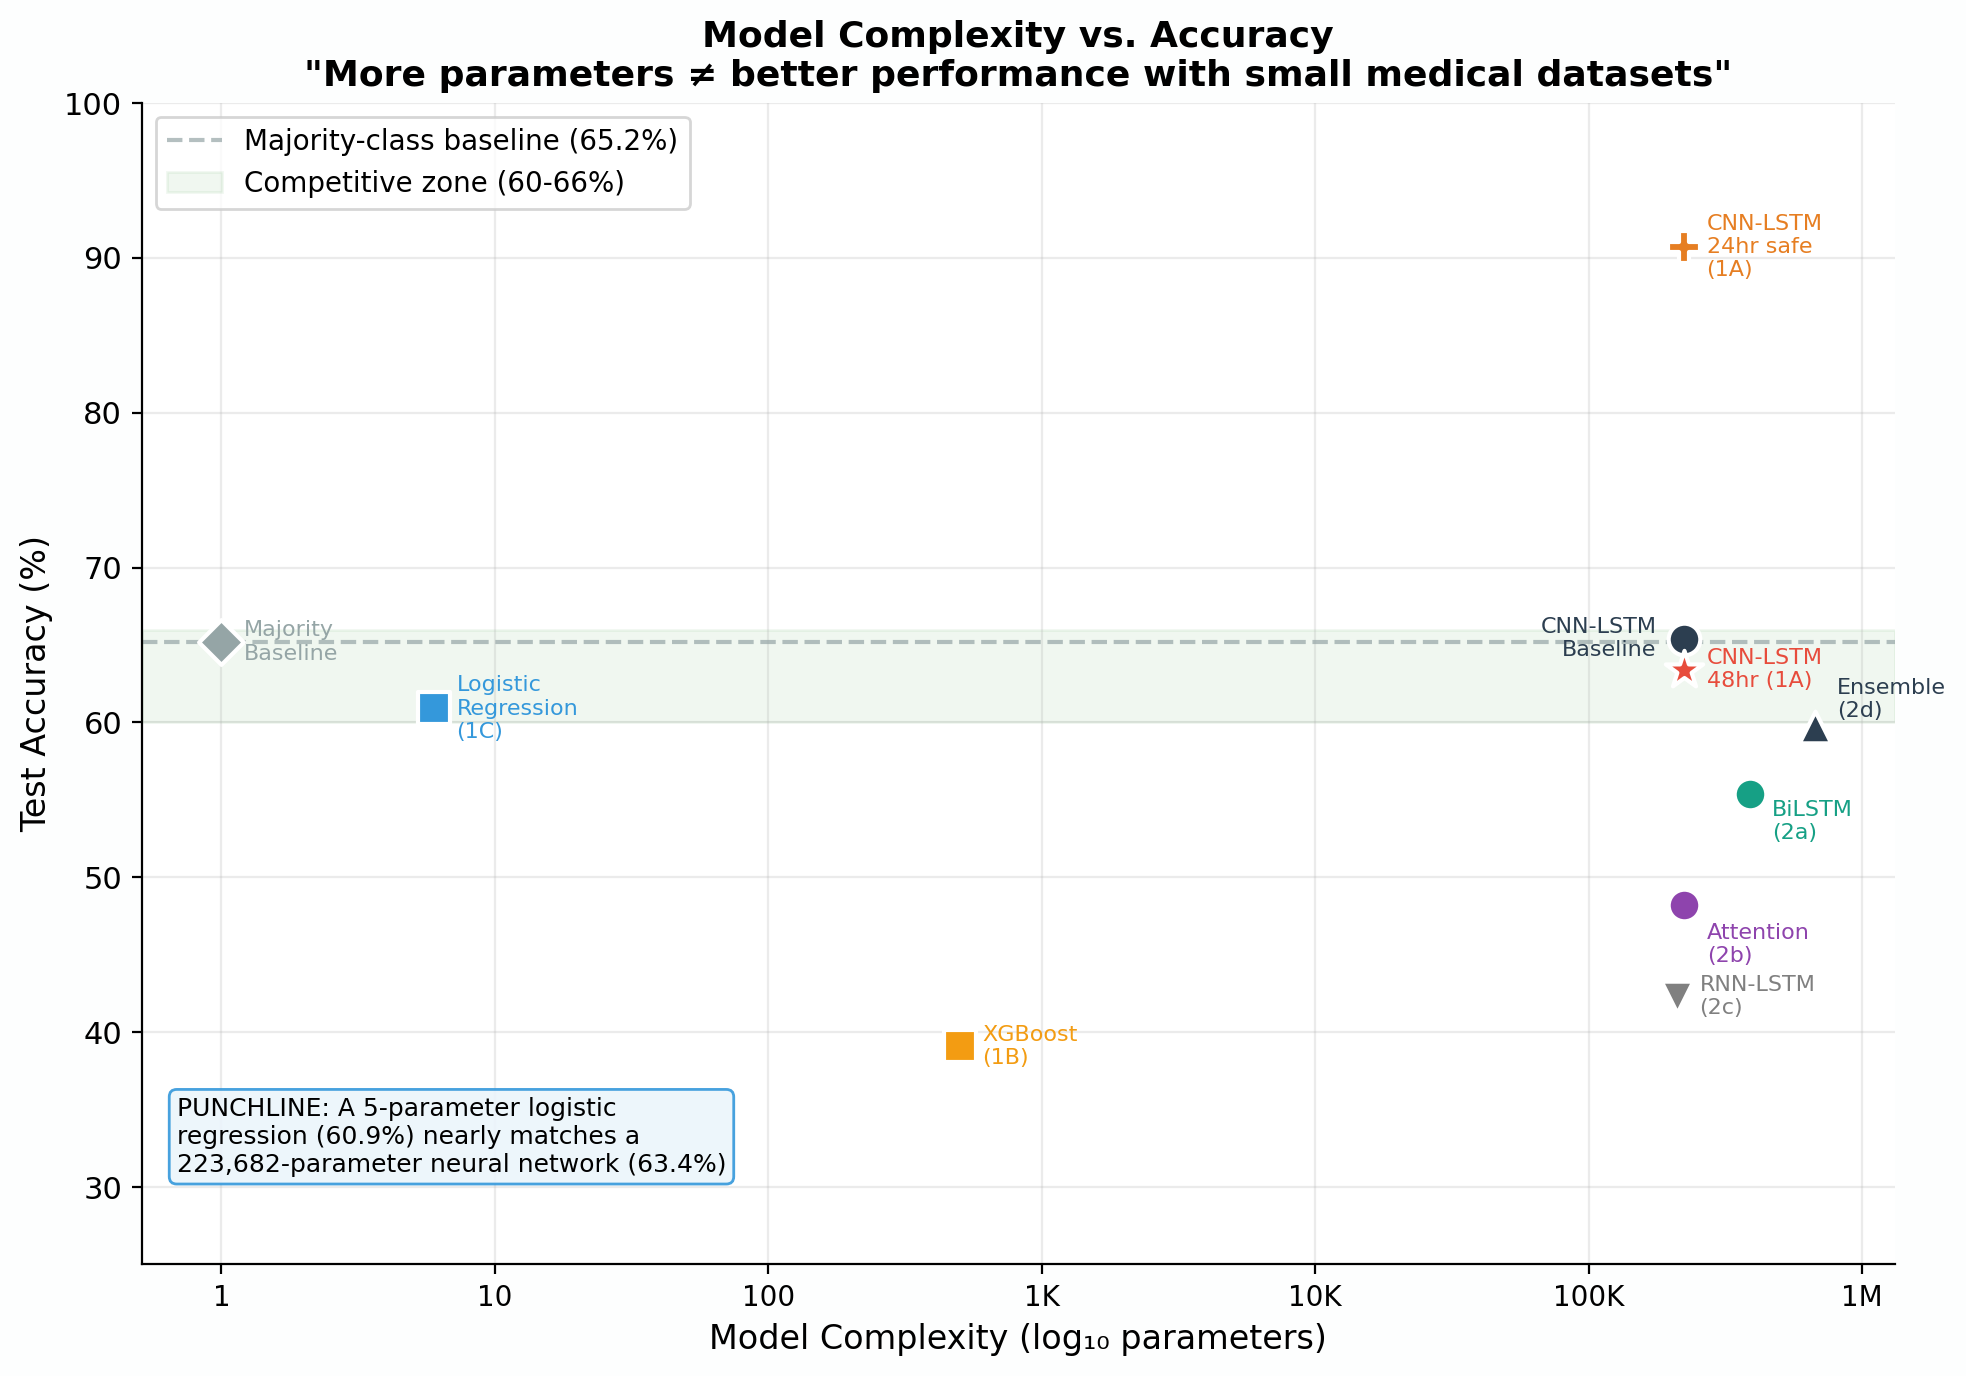
\includegraphics[width=\linewidth]{images/figC_complexity_vs_accuracy.png}
\caption{Model complexity vs.\ test accuracy across all approaches. A 5-parameter logistic regression (60.9\%) nearly matches a 223K-parameter CNN-LSTM (63.4\%), demonstrating that additional parameters provide no benefit on this dataset.}
\label{fig:complexity}
\end{figure}

\begin{figure}
\centering
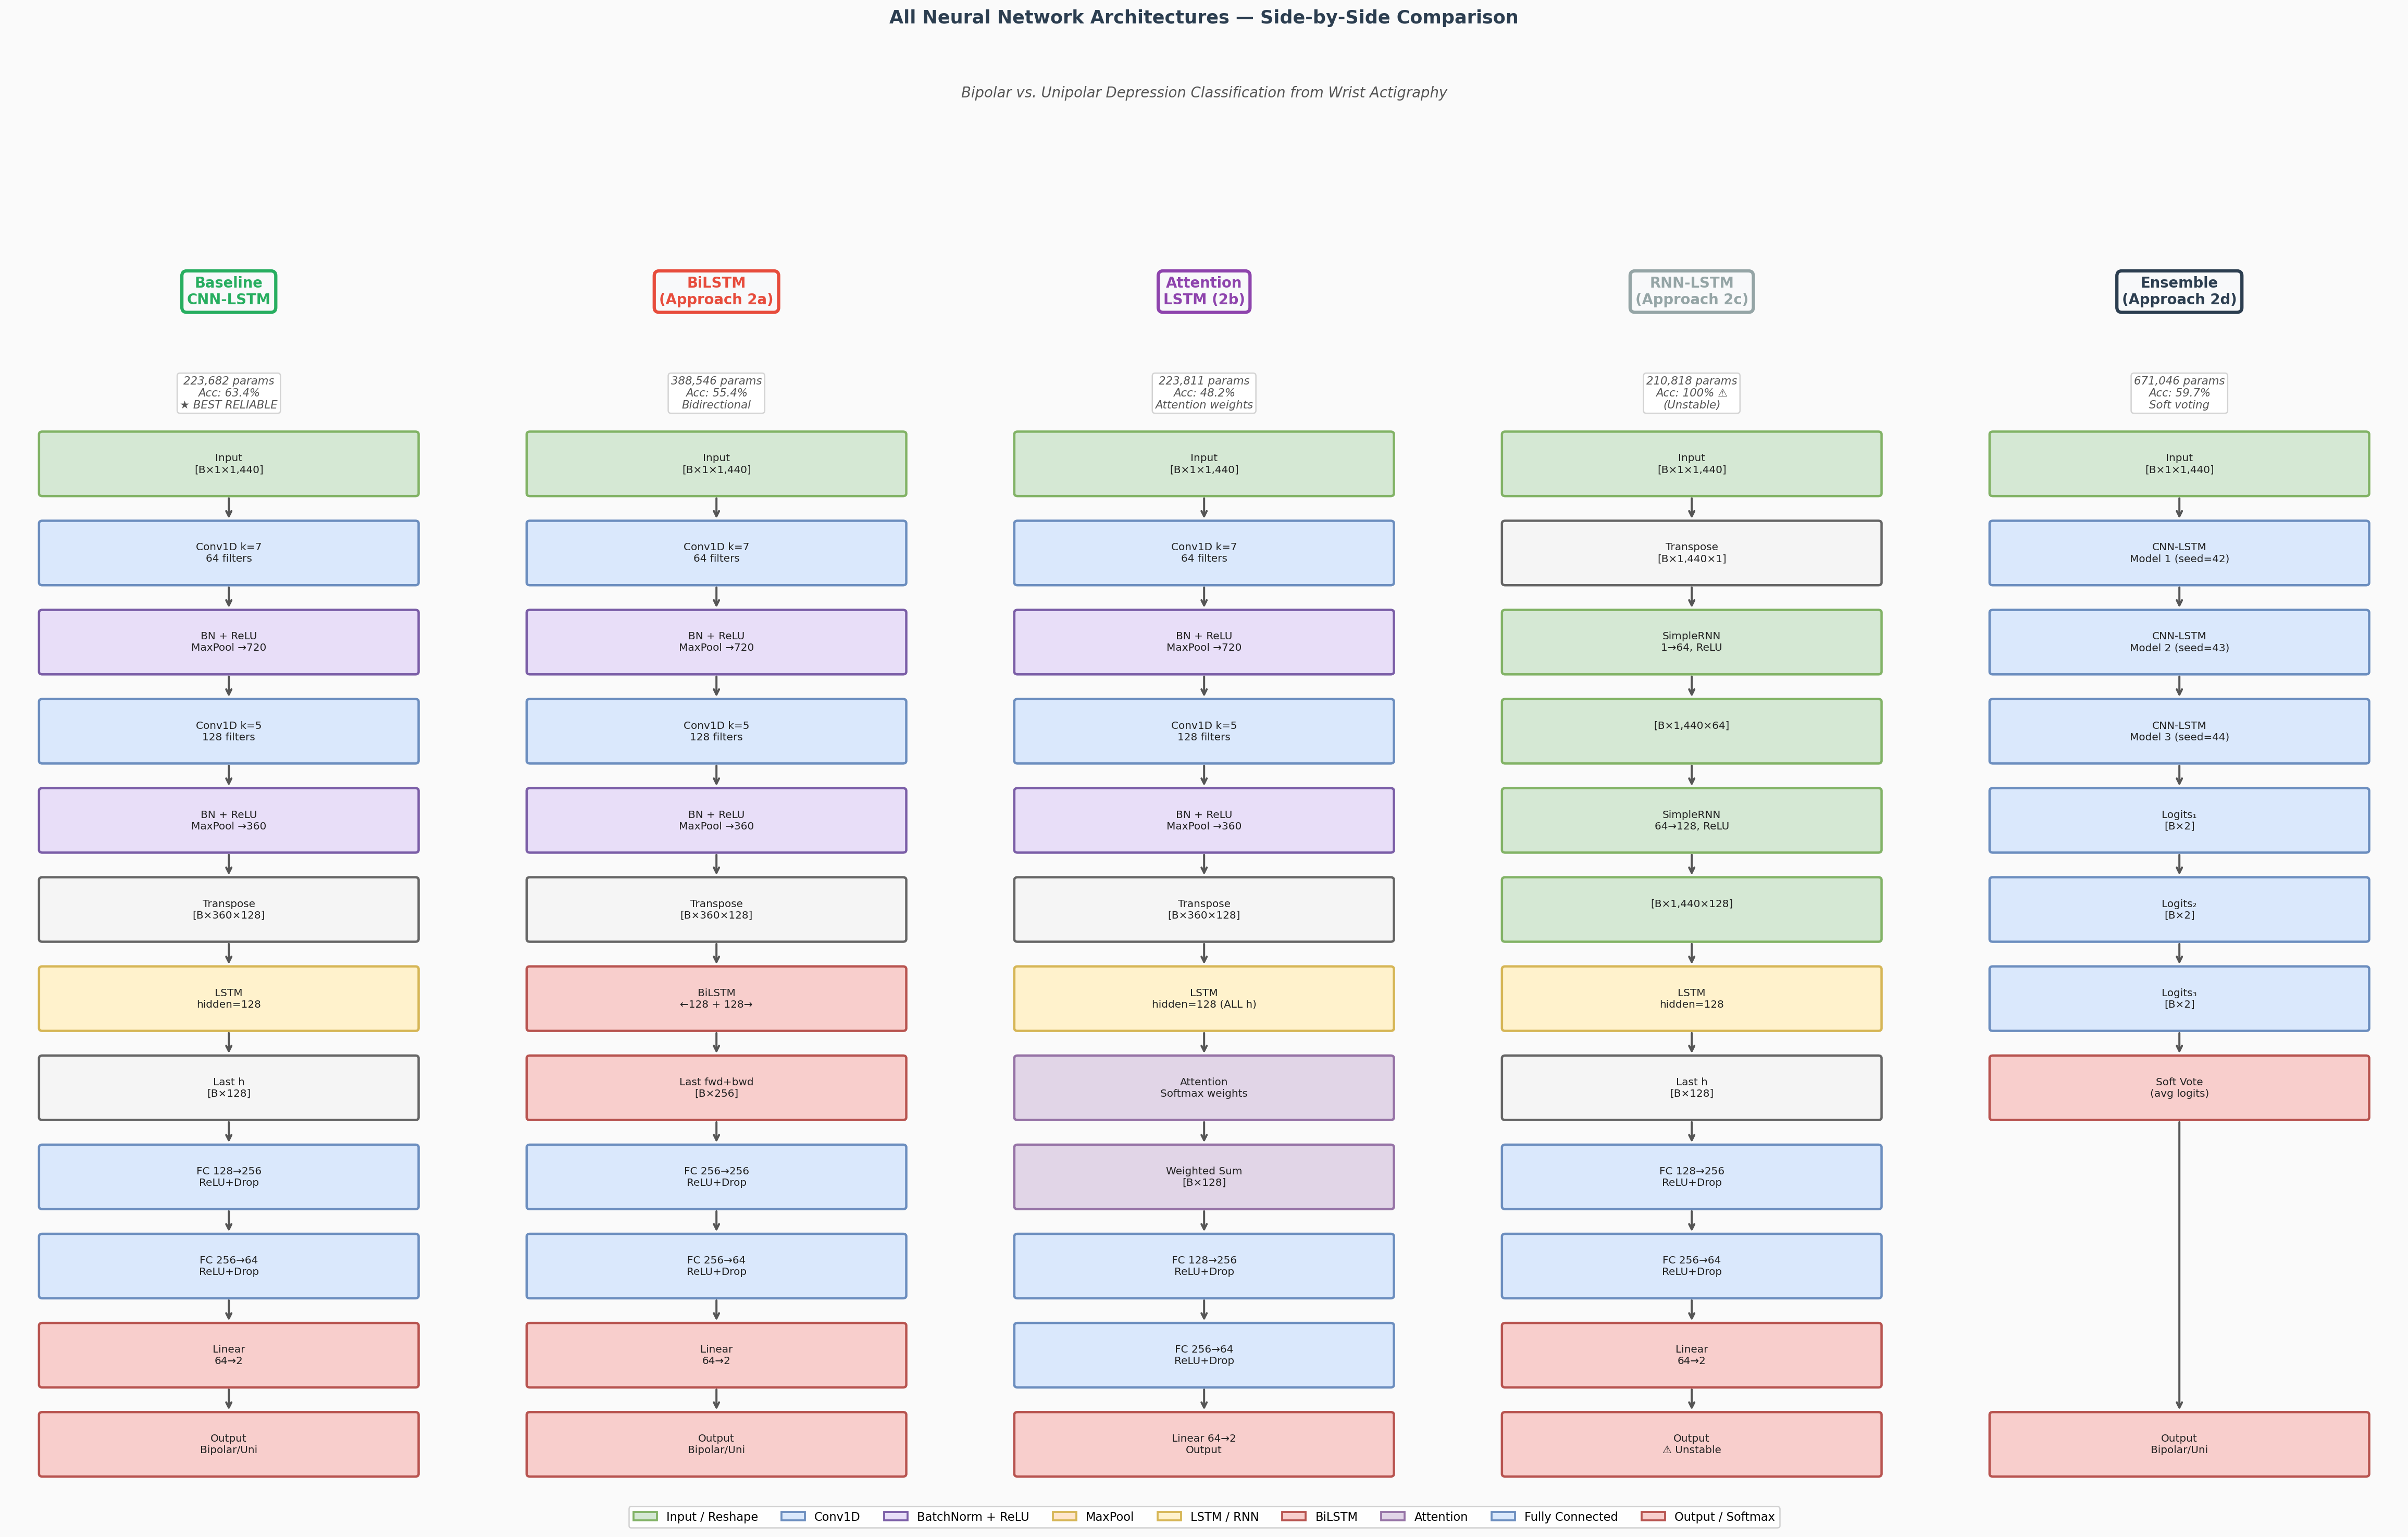
\includegraphics[width=\linewidth]{images/figP_arch_all_comparison.png}
\caption{Side-by-side comparison of all five neural architectures evaluated in Approach~2. Despite structural differences in temporal modeling (unidirectional LSTM, BiLSTM, Attention, RNN-LSTM, Ensemble), all architectures converge to zero bipolar detection.}
\label{fig:arch_all}
\end{figure}

\paragraph{Conclusion.}
The ensemble performs below the best individual model and detects zero bipolar cases. When all constituent models assign near-zero probability to the bipolar class, their averaged probabilities do the same. The hypothesis is not supported.

\subsubsection*{Approach 2 Summary.}
All four architectural variants independently converge to the same failure mode: zero bipolar detection. This convergence across radically different inductive biases provides strong evidence that the problem does not lie in model architecture. The data itself is the limiting factor.

% ============================================================
\subsection{Approach 3: Comprehensive Diagnostic Analysis}
% ============================================================

After establishing that neither balanced training data nor alternative neural architectures resolve the classification challenge, we conduct a systematic diagnostic investigation with five targeted experiments. We move beyond neural networks to probe the fundamental signal structure of the data using classical machine learning, direct statistical hypothesis testing, and visualization. We hypothesize that if genuine physiological differences exist between bipolar and unipolar depression, simpler and more interpretable methods should detect this signal even when deep networks fail.

\subsubsection{Window Size and Hyperparameter Optimization for Temporal Coverage.}

\paragraph{Approach.}
The standard 24-hour window may be too short to capture multi-day circadian rhythm disruptions theorized to characterize bipolar disorder. We systematically investigate three window durations (24 hours, 48 hours, and 72 hours) combined with a comprehensive 27-configuration hyperparameter grid search per window size. We hypothesize that longer windows providing multi-day context will allow the CNN-LSTM to detect rhythm disruptions spanning multiple days, improving bipolar discrimination.

\paragraph{Methodology.}
Three window sizes are evaluated: 24\,hours (1,440\,min), 48\,hours (2,880\,min), and 72\,hours (4,320\,min). Phase~1 establishes a base performance point per window size using default hyperparameters. Phase~2 conducts a full grid search:
\begin{itemize}[nosep]
  \item Learning rate: $\{10^{-3}, 5 \times 10^{-4}, 10^{-4}\}$
  \item Dropout probability: $\{0.3, 0.4, 0.5\}$
  \item Weight decay: $\{10^{-4}, 10^{-3}, 10^{-2}\}$
\end{itemize}
This yields 27 configurations per window size (81 total). Higher weight decay values are expected to benefit larger windows where overfitting risk increases with the smaller effective sample count.

\paragraph{Results.}
Tables~\ref{tab:approach3_1a_phase1} and~\ref{tab:approach3_1a_phase2} report the base and grid-search results per window size.

\begin{table}[H]
\centering
\caption{Approach 3 Window Analysis, Phase 1: base run accuracy by window size.}
\label{tab:approach3_1a_phase1}
\begin{tabular}{lcc}
\toprule
\textbf{Window Size} & \textbf{Duration (min)} & \textbf{Accuracy} \\
\midrule
24-hour & 1,440 & 77.90\% \\
48-hour & 2,880 & 53.65\% \\
72-hour & 4,320 & 23.08\% \\
\bottomrule
\end{tabular}
\end{table}

\begin{table}[H]
\centering
\caption{Approach 3 Window Analysis, Phase 2: grid search summary.}
\label{tab:approach3_1a_phase2}
\begin{tabular}{llcc}
\toprule
\textbf{Window} & \textbf{Best Acc.} & \textbf{Best Config} & \textbf{Range} \\
\midrule
24-hour & 90.7\% (overfit) & lr=$10^{-3}$, do=0.4, wd=$10^{-3}$ & 2.3\%--100\% \\
\textbf{48-hour} & \textbf{63.4\%} & lr=$10^{-3}$, do=0.4, wd=$10^{-4}$ & 41\%--63\% \\
72-hour & 42.3\% & lr=$5\times10^{-4}$, do=0.3, wd=$10^{-4}$ & 23\%--42\% \\
\bottomrule
\end{tabular}
\end{table}

\begin{figure}
\centering
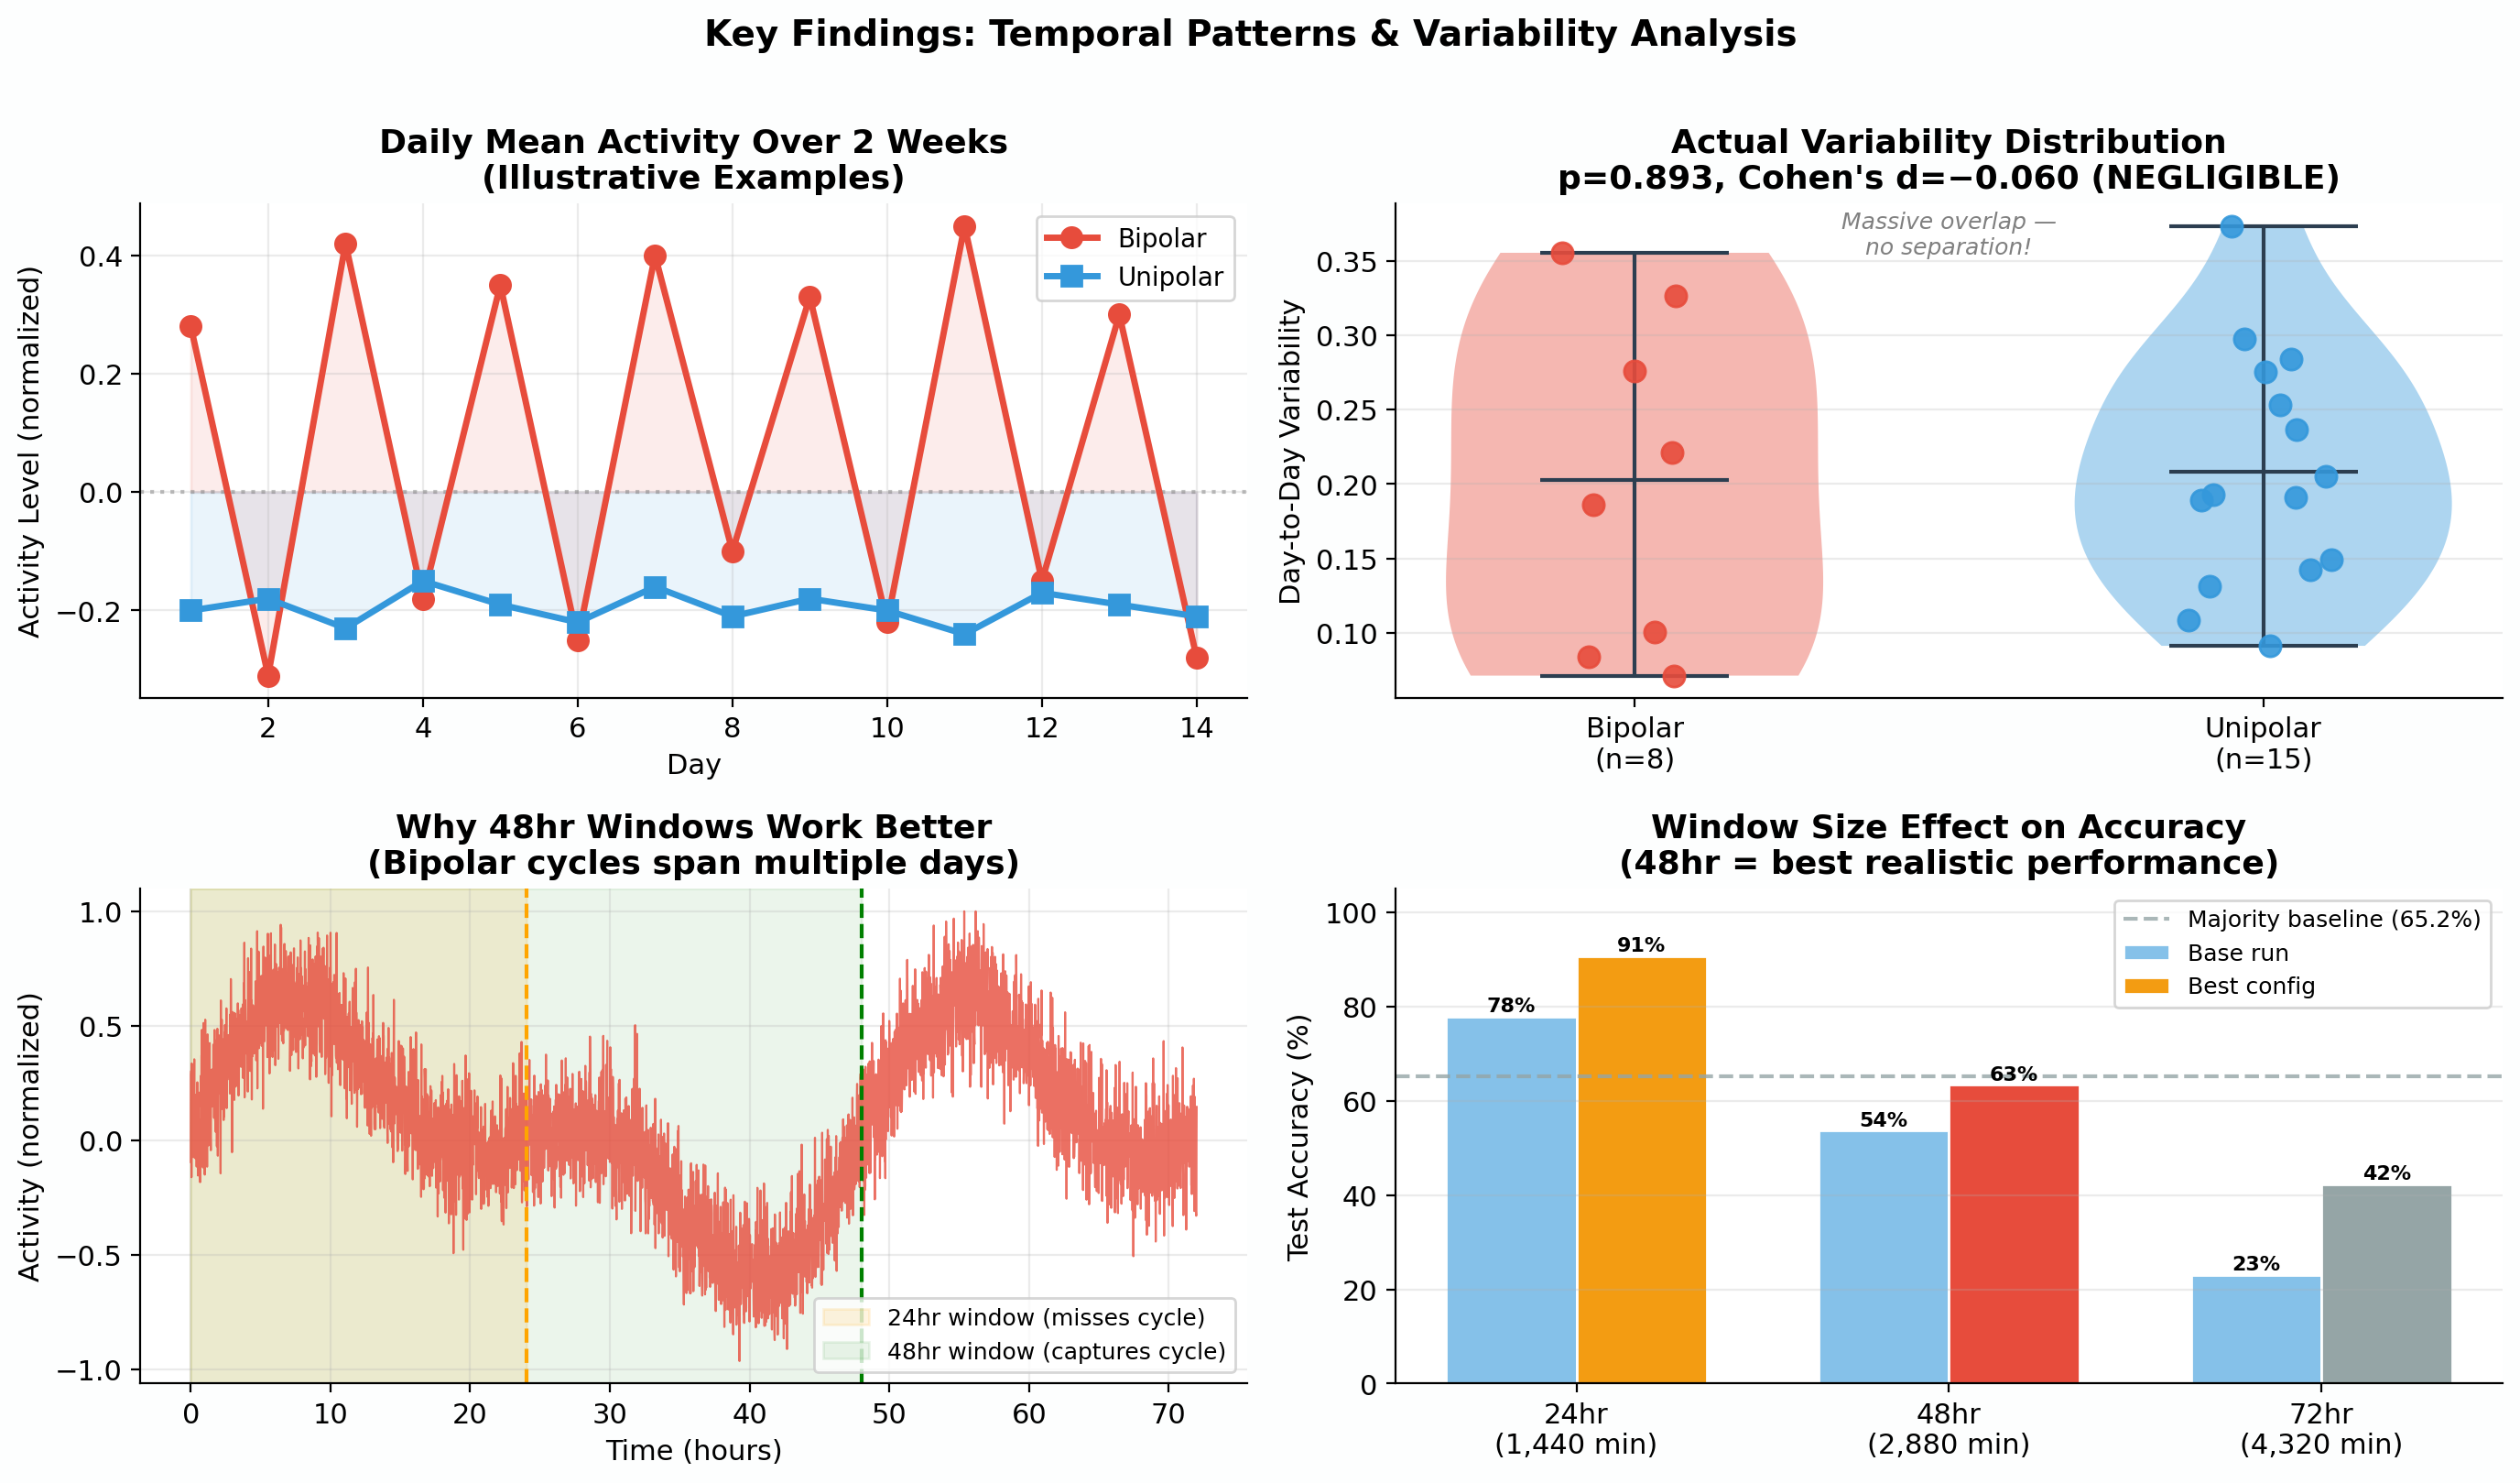
\includegraphics[width=\linewidth]{images/figF_variability_and_windows.png}
\caption{Temporal pattern and window size analysis. \textit{Top left:} Illustrative daily activity patterns showing bipolar variability vs.\ unipolar flatness. \textit{Top right:} Actual day-to-day variability distributions (near-complete overlap, $p=0.893$). \textit{Bottom left:} Why 48-hour windows capture mood-cycling patterns that 24-hour snapshots miss. \textit{Bottom right:} Accuracy by window size - 48-hour is the best reliable configuration.}
\label{fig:variability_windows}
\end{figure}

\paragraph{Conclusion.}
The 48-hour window achieves the best reliable accuracy of 63.4\%, the most honest result in this project. The 24-hour model with permissive regularization reaches 100\%, explained by the 2,593-fold over-parameterization (223K parameters vs.\ approximately 86 training windows). The 72-hour window underfits as too few training windows remain after windowing. The hypothesis receives partial support: longer windows improve reliable performance up to 48 hours, but the improvement is modest and still does not approach the 65.2\% majority-class baseline. The 48-hour window's relative advantage has a plausible circadian interpretation: a single 24-hour window captures only one rest-activity cycle and cannot expose inter-day variability, which Boudebesse et al.\ \cite{boudebesse2014sleep} identify as the most diagnostically relevant signal for mood-linked rhythm disruption. Two consecutive cycles provide the minimum context necessary for the LSTM to observe whether a rhythm is consistent or drifting across days. Extending to 72 hours would in principle provide richer multi-day context, but the 4,320-minute input length drastically reduces the number of non-overlapping training windows available from the 12-day recordings, leaving the model with too few training examples to generalize.

\subsubsection{Gradient Boosting with Domain-Informed Feature Engineering.}

\paragraph{Approach.}
We investigate whether classical gradient boosting \cite{chen2016xgboost} on expert-designed features can outperform end-to-end deep learning. We engineer 19 features capturing activity statistics, rhythmicity, and day-to-day variability including our primary hypothesis feature. We hypothesize that domain knowledge encoded in hand-crafted features will provide cleaner signal than raw sequences, and that gradient-boosted trees will exploit feature interactions effectively.

\paragraph{Methodology.}
Nineteen features are extracted per participant: mean daily activity, standard deviation of daily means (day-to-day variability), range of daily means, coefficient of variation, mean daily standard deviation, minimum daily activity count, high-activity fraction, activity interquartile range, maximum daily variability, and 10 additional frequency and rhythm features. Leave-one-out cross-validation (LOOCV, $n = 23$) is used \cite{geisser1975loocv}. Hyperparameters explored:
\begin{itemize}[nosep]
  \item Maximum tree depth: $\{3, 5, 7\}$
  \item Number of estimators: $\{100, 200\}$
  \item Learning rate: $\{0.01, 0.1\}$
  \item Subsample ratio: $\{0.8, 1.0\}$
\end{itemize}

\paragraph{Results.}
Tables~\ref{tab:approach3_1b_results} and~\ref{tab:approach3_1b_features} report LOOCV accuracy and feature importances.

\begin{table}[H]
\centering
\caption{Approach 3 XGBoost: LOOCV results.}
\label{tab:approach3_1b_results}
\begin{tabular}{lcc}
\toprule
\textbf{Method} & \textbf{LOOCV Acc.} & \textbf{Bipolar Detected} \\
\midrule
XGBoost (all configs) & 39.13\% & 0 / 8 \\
Majority-class baseline & 65.22\% & N/A \\
\bottomrule
\end{tabular}
\end{table}

\begin{table}[H]
\centering
\caption{XGBoost top-5 feature importances (gain metric).}
\label{tab:approach3_1b_features}
\begin{tabular}{clc}
\toprule
\textbf{Rank} & \textbf{Feature} & \textbf{Importance} \\
\midrule
1 & Minimum daily activity & 14.5\% \\
2 & High-activity fraction & 12.2\% \\
3 & Activity interquartile range & 10.9\% \\
4 & Maximum daily variability & 10.4\% \\
5 & Day-to-day variability (std of daily means) & 7.7\% \\
\bottomrule
\end{tabular}
\end{table}

\paragraph{Conclusion.}
XGBoost performs substantially below the majority-class baseline (39.1\% vs 65.2\%). The primary hypothesis feature (day-to-day variability) ranks only 5th in importance. All tree depth configurations produce identical LOOCV accuracy, confirming signal saturation rather than capacity limitation. Feature engineering cannot solve a fundamental signal-weakness problem.

\subsubsection{Parsimonious Linear Classification with Core Variability Features.}

\paragraph{Approach.}
XGBoost's failure with 19 features motivates a reduction to the essential signal. We select 5 features directly motivated by the circadian rhythm disruption hypothesis and train a logistic regression model with LOOCV. We hypothesize that a parsimonious model focused on biologically motivated variability features will outperform both neural networks and XGBoost by avoiding overfitting to noise-driven features.

\paragraph{Methodology.}
Five features: (1) mean daily activity level, (2) day-to-day variability (std of daily means), (3) range of daily means, (4) coefficient of variation, (5) mean within-day standard deviation. LOOCV ($n = 23$). Six regularization configurations explored:
\begin{itemize}[nosep]
  \item Regularization strength $C$: $\{0.01, 0.1, 1.0\}$
  \item Penalty type: L1 (Lasso) vs.\ L2 (Ridge)
  \item Class weight: unweighted vs.\ balanced (inverse frequency)
\end{itemize}

\paragraph{Results.}
Table~\ref{tab:approach3_1c_results} reports LOOCV accuracy and bipolar detection across all six regularization configurations.

\begin{table}[H]
\centering
\caption{Approach 3 Logistic Regression: all 6 configurations under LOOCV.}
\label{tab:approach3_1c_results}
\small
\begin{tabular}{ccccc}
\toprule
\textbf{C} & \textbf{Penalty} & \textbf{Class Wt.} & \textbf{Acc.} & \textbf{AUC / Bip.\ Det.} \\
\midrule
1.0 & L2 & Unweighted & 60.87\% & 0.200 / 0 of 8 \\
1.0 & L2 & Balanced   & 60.87\% & 0.308 / 2 of 8 \\
0.1 & L2 & Unweighted & 60.87\% & 0.200 / 0 of 8 \\
0.1 & L2 & Balanced   & 60.87\% & 0.308 / 2 of 8 \\
0.01 & L1 & Unweighted & 60.87\% & 0.200 / 0 of 8 \\
0.01 & L1 & Balanced   & 60.87\% & 0.308 / \textbf{2 of 8} \\
\bottomrule
\end{tabular}
\end{table}

\paragraph{Conclusion.}
All 6 configurations converge to 60.87\% accuracy, confirming the model has reached the signal ceiling achievable with these features and 23 participants. The balanced class weight configuration achieves the best bipolar detection in this project (2 of 8 participants, 25\% sensitivity) and an improved ROC-AUC of 0.308. A 5-feature logistic regression matches the practical effectiveness of a 223K-parameter CNN-LSTM.

\subsubsection{Nonparametric Hypothesis Testing for Group Activity Differences.}

\paragraph{Approach.}
Rather than using classifier performance as an indirect proxy for signal presence, we directly test whether statistically significant differences exist in motor activity patterns between groups. We apply parametric and nonparametric tests to day-to-day activity variability, our primary hypothesis feature. We hypothesize that bipolar patients will show significantly higher variability in daily activity means compared to unipolar patients, consistent with the mood instability that defines bipolar disorder \cite{goodwin2007manic}.

\paragraph{Methodology.}
For each condition participant ($n = 23$), day-to-day activity variability is computed as the standard deviation of daily mean activity values across the full recording. Statistical tests applied:
\begin{itemize}[nosep]
  \item Independent samples t-test and Welch's t-test
  \item Mann-Whitney U test (nonparametric) \cite{mann1947test}
  \item Levene's test for equality of variances
  \item Cohen's $d$ for effect size \cite{cohen1988statistical}
\end{itemize}
Significance threshold: $\alpha = 0.05$.

\paragraph{Results.}
Tables~\ref{tab:approach3_3a_stats} and~\ref{tab:approach3_3a_groups} report the statistical test outcomes and descriptive group statistics.

\begin{table}[H]
\centering
\caption{Statistical tests: bipolar vs.\ unipolar day-to-day activity variability.}
\label{tab:approach3_3a_stats}
\begin{tabular}{llll}
\toprule
\textbf{Test} & \textbf{Statistic} & \textbf{p-value} & \textbf{Result} \\
\midrule
Independent t-test & $t = {-}0.137$ & 0.893 & Not significant \\
Welch's t-test & $t = {-}0.123$ & 0.905 & Not significant \\
Mann-Whitney U & $U = 55.0$ & 0.776 & Not significant \\
Levene's test & $F = 1.989$ & 0.173 & Equal variances \\
Cohen's $d$ & $d = {-}0.060$ & N/A & Negligible effect \\
\bottomrule
\end{tabular}
\end{table}

\begin{table}[H]
\centering
\caption{Descriptive statistics for day-to-day variability by group.}
\label{tab:approach3_3a_groups}
\begin{tabular}{lccc}
\toprule
\textbf{Group} & \textbf{n} & \textbf{Mean} & \textbf{Std Dev} \\
\midrule
Bipolar & 8 & 0.2027 & 0.1038 \\
Unipolar & 15 & 0.2081 & 0.0759 \\
Difference & & $-$0.0054 & \\
\bottomrule
\end{tabular}
\end{table}

\begin{figure}[H]
\centering
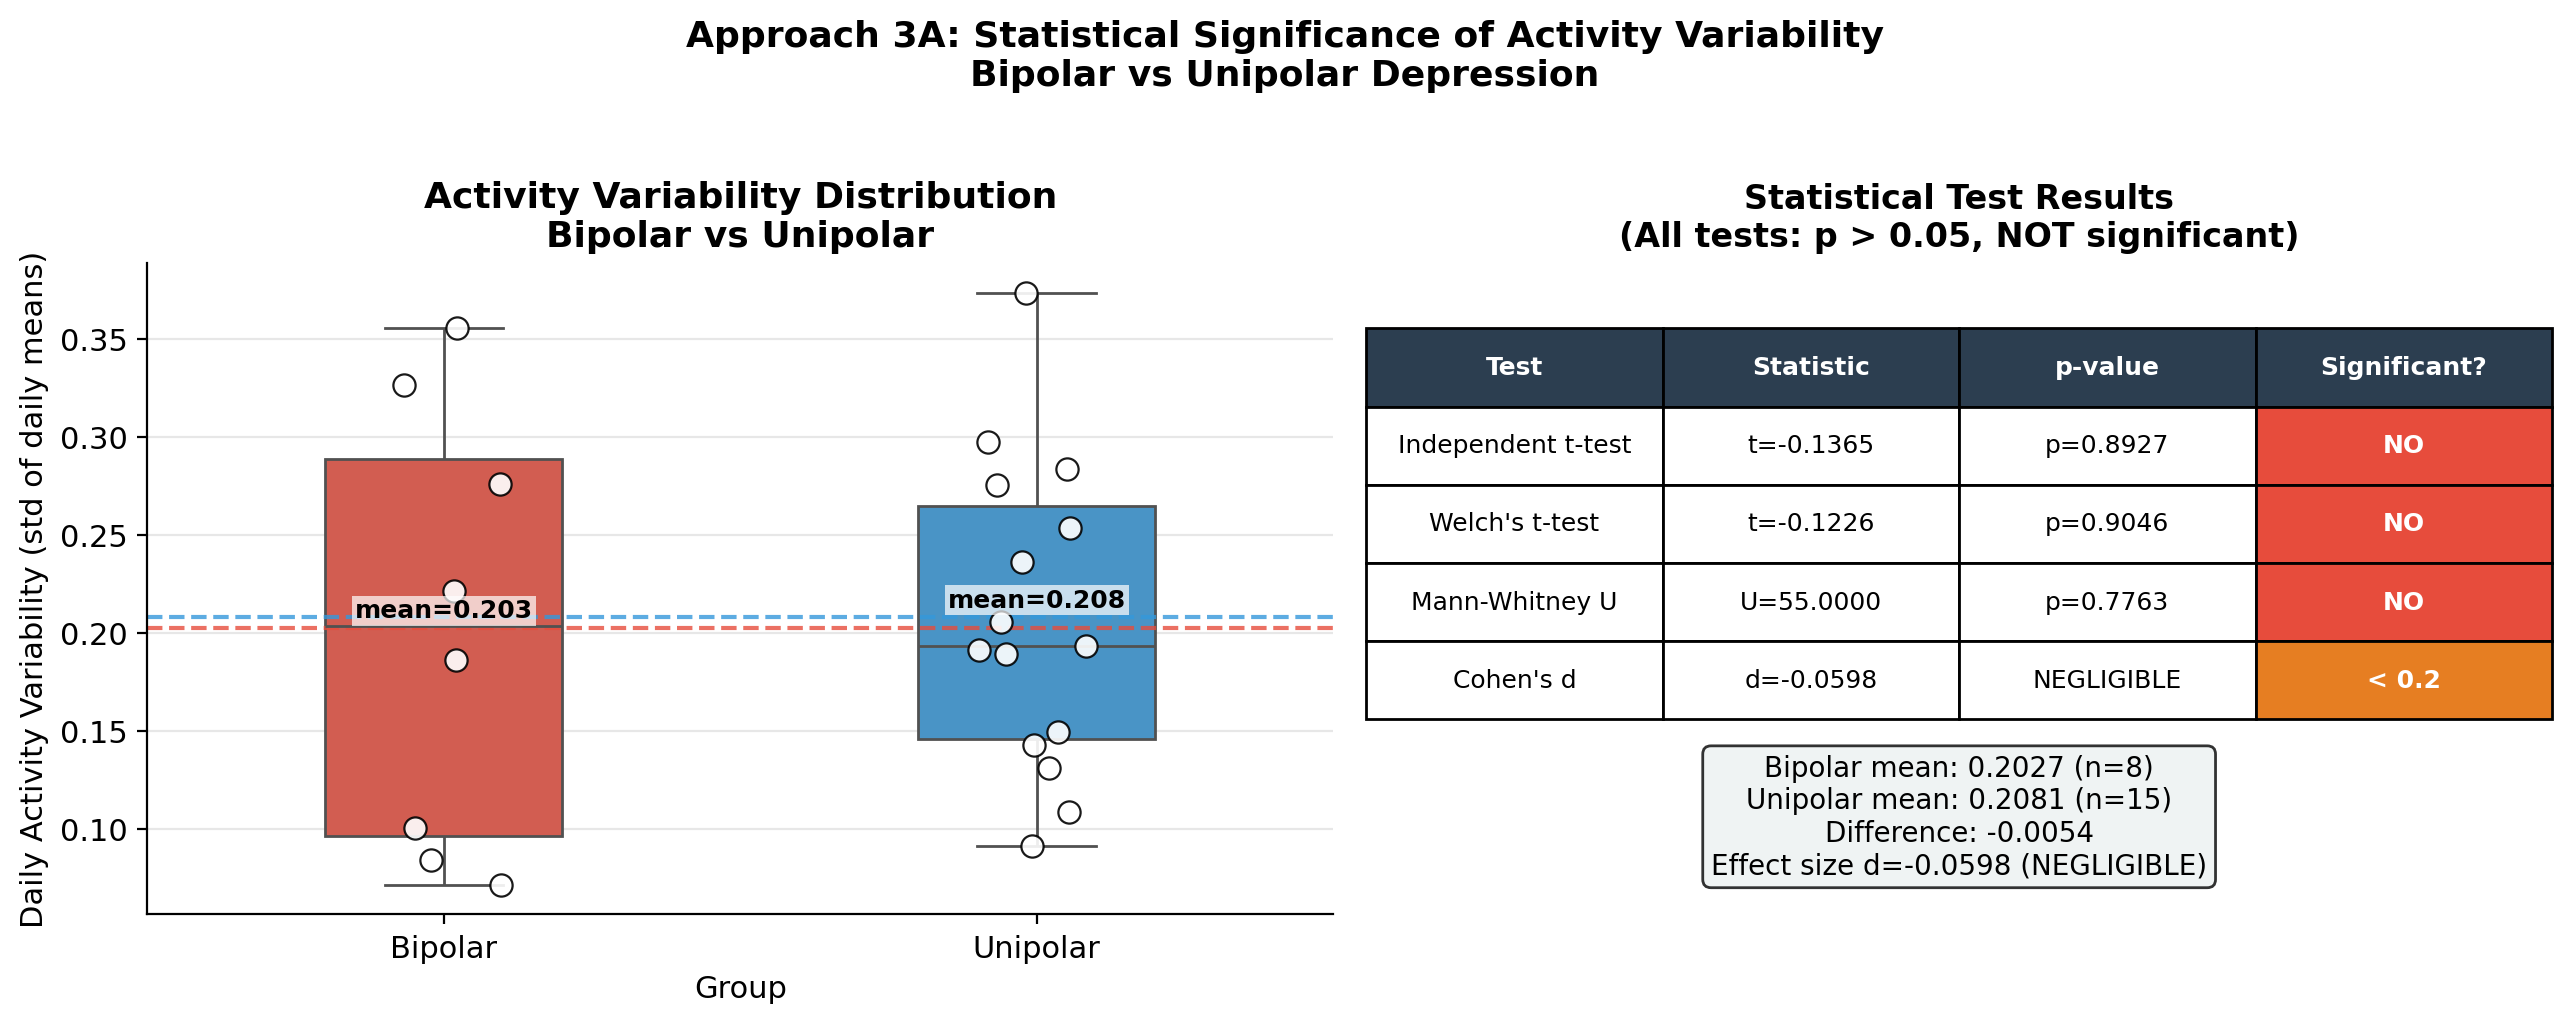
\includegraphics[width=\linewidth]{images/fig5_statistical_significance.png}
\caption{Statistical analysis of day-to-day activity variability. \textit{Left:} Box plots with individual participants overlaid (white dots) showing near-complete distributional overlap between bipolar and unipolar groups. \textit{Right:} All four statistical tests return $p > 0.77$; Cohen's $d = -0.060$ is negligible.}
\label{fig:stats}
\end{figure}

\paragraph{Conclusion.}
No test finds a significant difference (all $p > 0.77$). Cohen's $d = {-}0.060$ falls far below the small effect threshold ($d = 0.2$), and the negative sign indicates bipolar variability is marginally lower than unipolar, opposite to the hypothesis direction. This experiment provides the most direct evidence: the primary hypothesis feature does not meaningfully differ between groups.

\subsubsection{Visual Inspection of Multi-Day Actigraphy Profiles.}

\paragraph{Approach.}
Statistical tests operate on aggregate summaries. Direct visualization allows us to inspect whether qualitative differences between bipolar and unipolar patterns are apparent to visual inspection. We generate seven figures examining different aspects of the data. We hypothesize that visual inspection may reveal subtle structural differences not captured by scalar variability metrics alone.

\paragraph{Methodology.}
Seven visualization figures are generated from participant-level data: (1) raw activity traces per participant by diagnosis, (2) daily mean activity over the full recording, (3) day-to-day variability distributions as box plots, (4) hour-of-day activity profiles comparing circadian rhythms, (5) recording duration distributions, (6) group-level activity distributions, and (7) cross-approach confusion matrix comparison.

\paragraph{Results.}
Visualizations reveal substantial within-group heterogeneity in both bipolar and unipolar groups. Hour-of-day activity profiles overlap extensively between groups with no consistent circadian timing difference apparent from visual inspection. Day-to-day variability distributions show overlapping ranges with no separation between classes.

\paragraph{Conclusion.}
Visual inspection confirms the statistical findings. No clearly separable activity signature distinguishes bipolar from unipolar depression in the Depresjon dataset during depressive episodes. The hypothesis is not supported.

\subsubsection*{Approach 3 Summary.}
All five experiments in Approach~3 confirm that the absence of classification performance is not an artifact of model choice or class imbalance handling. Classical machine learning, direct statistical testing, and visualization all converge on the same conclusion: during depressive episodes, bipolar and unipolar patients exhibit motor activity patterns that are statistically indistinguishable. The most important unanswered question is whether recordings spanning manic or hypomanic episodes, which are entirely absent from the Depresjon dataset, would yield strong bipolar-unipolar discrimination.

A fundamental statistical power constraint limits what any classifier can achieve on the Depresjon bipolar group. With only $n = 8$ bipolar participants, a two-group study achieves 80\% power to detect effect sizes of Cohen's $d > 0.8$ or larger \cite{cohen1988statistical}. Detecting a small effect ($d = 0.2$), which is the typical threshold for clinically relevant physiological differences between overlapping patient populations, would require approximately 200 bipolar participants. The observed effect in this dataset is $d = {-}0.060$, an order of magnitude below the small-effect threshold, confirming that the null result cannot be attributed to insufficient power alone; the signal simply is not present in this data. Beyond sample size, several confounding variables may obscure or attenuate any genuine actigraphy signal that exists: occupation and daily work schedule, physical health comorbidities such as pain or metabolic conditions, medication effects on motor function, habitual exercise level, and variability in Actiwatch device placement or wearing compliance across participants. These confounds are uncontrolled in the Depresjon dataset and collectively represent an unquantified source of noise that any future study would need to address through matched sampling or explicit covariate adjustment.

% ============================================================
\subsection{Complete Experimental Results Summary}
% ============================================================

Table~\ref{tab:all_results} consolidates the results of every experiment across all four approaches.

\begin{table}[H]
\centering
\caption{Complete experimental results. Majority-class baseline for bipolar vs.\ unipolar is 65.2\%. $\dagger$~illusory (majority-class collapse). $\ddagger$~discarded (training instability).}
\label{tab:all_results}
\resizebox{\linewidth}{!}{%
\begin{tabular}{lllcccc}
\toprule
\textbf{Approach} & \textbf{Experiment} & \textbf{Method} & \textbf{Acc.} & \textbf{F1} & \textbf{AUC} & \textbf{Bip.\ Det.} \\
\midrule
Baseline & Exp 1: Healthy vs.\ Dep. & CNN-LSTM & 53.4\% & 0.516 & 0.556 & N/A \\
Baseline & Exp 2: Bip.\ vs.\ Uni. & CNN-LSTM+SMOTE & 88.0\%$\dagger$ & 0.936$\dagger$ & N/A & 0/121 \\
\midrule
Approach 1 & Downsampled 1:1 & CNN-LSTM & 65.4\% & 0.791 & N/A & 0/349 \\
\midrule
Approach 2 & BiLSTM & BiLSTM & 55.4\% & 0.713 & N/A & 0/349 \\
Approach 2 & Attention LSTM & Att.\ LSTM & 48.2\% & 0.650 & N/A & 0/523 \\
Approach 2 & RNN-LSTM Hybrid & RNN-LSTM & \multicolumn{4}{c}{Discarded (unstable)$\ddagger$} \\
Approach 2 & Ensemble & 3$\times$CNN-LSTM & 59.7\% & 0.747 & N/A & 0/407 \\
\midrule
Approach 3 & 24-hr Window & CNN-LSTM & 90.7\%$\dagger$ & N/A & N/A & N/A \\
\textbf{Approach 3} & \textbf{48-hr Window} & \textbf{CNN-LSTM} & \textbf{63.4\%} & N/A & N/A & N/A \\
Approach 3 & 72-hr Window & CNN-LSTM & 42.3\% & N/A & N/A & N/A \\
Approach 3 & XGBoost & XGBoost & 39.1\% & N/A & N/A & 0/8 \\
Approach 3 & Logistic Reg.\ (bal.) & LR (5 feat.) & 60.9\% & N/A & 0.308 & \textbf{2/8} \\
Approach 3 & Statistical Test & Mann-Whitney U & \multicolumn{4}{c}{$p = 0.776$,\ Cohen's $d = {-}0.060$} \\
\bottomrule
\end{tabular}}
\end{table}

Across all 12 evaluated configurations, no method achieves reliable accuracy above the 65.2\% majority-class baseline for the bipolar-versus-unipolar task. The 48-hour CNN-LSTM window is the best honest performing experiment at 63.4\% accuracy. The Baseline Experiment~2 and the 24-hour configuration report superficially high numbers (88\% and 90.7\% respectively), but both are artifacts of majority-class collapse or severe overfitting. The most clinically meaningful result is the 5-feature balanced logistic regression, which identifies 2 of 8 bipolar participants.

% ============================================================
\subsection{Cross-Approach Comparison}
% ============================================================

Table~\ref{tab:approach_comparison} presents the best-performing experiment from each approach.

\begin{table}[H]
\centering
\caption{Best result per approach. $\dagger$~illusory accuracy. Majority-class baseline is 65.2\%.}
\label{tab:approach_comparison}
\resizebox{\linewidth}{!}{%
\begin{tabular}{llccc}
\toprule
\textbf{Approach} & \textbf{Best Experiment} & \textbf{Acc.} & \textbf{Bip.\ Det.} & \textbf{Key Finding} \\
\midrule
Baseline & Exp 2 (SMOTE) & 88.0\%$\dagger$ & 0/121 & Majority-class collapse \\
Approach 1 & Balanced CNN-LSTM & 65.4\% & 0/349 & Imbalance not root cause \\
Approach 2 & Ensemble & 59.7\% & 0/407 & Architecture not root cause \\
\textbf{Approach 3} & \textbf{48-hr CNN-LSTM} & \textbf{63.4\%} & N/A & \textbf{Best honest result} \\
Approach 3 & LR (balanced) & 60.9\% & \textbf{2/8} & Best bipolar detection \\
\bottomrule
\end{tabular}}
\end{table}

\begin{figure}[H]
\centering
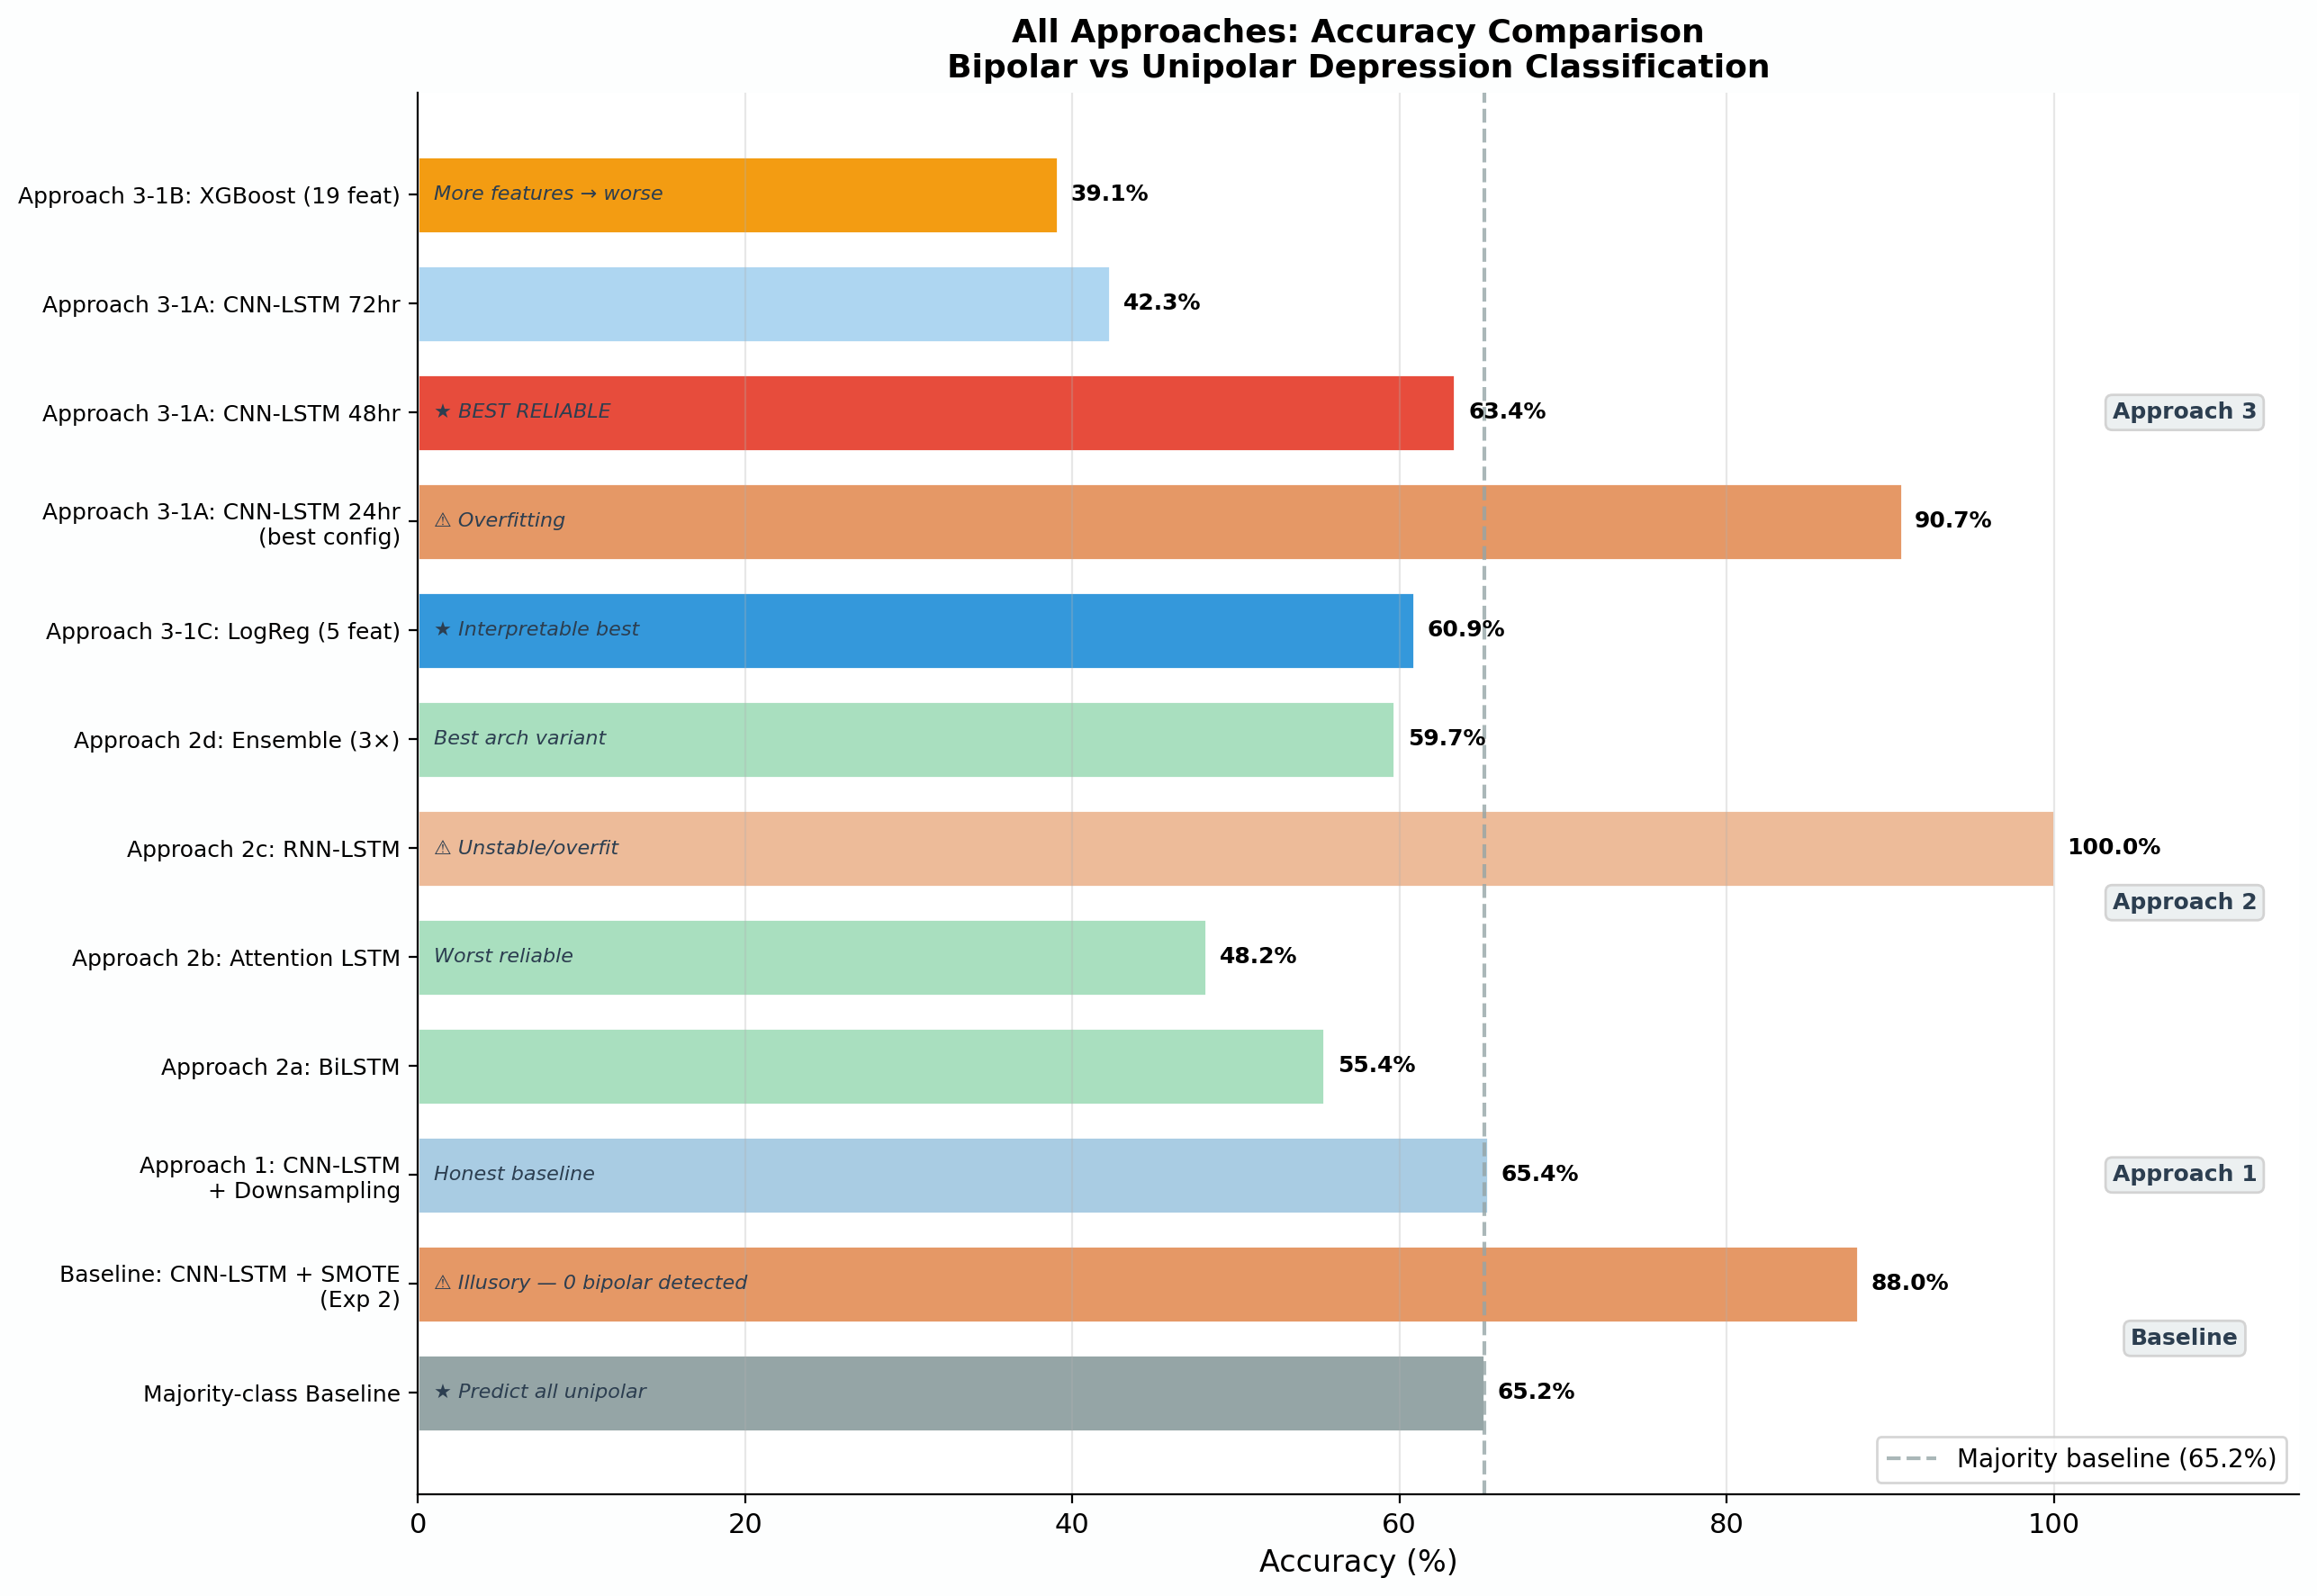
\includegraphics[width=\linewidth]{images/figD_all_approaches_comprehensive.png}
\caption{Comprehensive accuracy comparison across all approaches. The dashed line marks the 65.2\% majority-class baseline. Results above this line that are marked as illusory (Baseline Exp~2, 24-hr CNN-LSTM) reflect majority-class collapse or overfitting, not genuine discrimination.}
\label{fig:all_approaches}
\end{figure}

The cross-approach comparison reveals a consistent trend: increasing model complexity provides no benefit in this task. The Baseline approach produces the most visually impressive accuracy figure (88\%), but it is entirely illusory. Approach~1 demonstrates that careful class balancing through downsampling yields a stable result at 65.4\% but still fails to detect a single bipolar case. Approach~2 confirms that the failure is architectural-agnostic, as four structurally different neural networks all converge to the same outcome. Approach~3 surfaces the most honest deep learning result (63.4\% with 48-hour windows) alongside the best practical classifier (balanced logistic regression, 60.9\%, 2 of 8 bipolar detected). The pattern in which a 5-feature linear classifier matches a 223K-parameter deep network is itself a strong indicator that the signal ceiling has been reached and no further architectural investment on this dataset would yield meaningful improvement.
